% Client and server topology for the real-robot inference pipeline.
% Compile with `pdflatex inference_topology.tex` and rasterise with
% `pdftoppm -png -r 200 inference_topology.pdf inference_topology` to produce
% docs/img/inference_topology.png.
\documentclass[border=6pt]{standalone}
\usepackage[T1]{fontenc}
\usepackage{mathptmx}
\usepackage{tikz}
\usetikzlibrary{positioning, arrows.meta, calc, fit, backgrounds, shapes.symbols}

\definecolor{clientblue}{HTML}{3D7ABF}
\definecolor{servergreen}{HTML}{2E8B57}
\definecolor{linkgray}{HTML}{555555}
\definecolor{bgclient}{HTML}{F0F4FA}
\definecolor{bgserver}{HTML}{EFF7F1}

\begin{document}
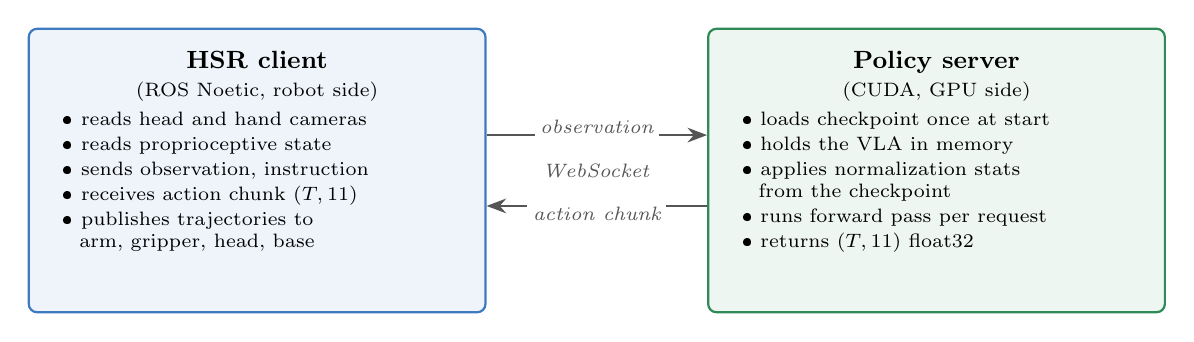
\begin{tikzpicture}[
    >=Stealth,
    font=\footnotesize,
    node distance=0.35cm and 0.5cm,
    clientbox/.style={
        draw=clientblue, fill=clientblue!8, rounded corners=3pt,
        minimum width=5.8cm, minimum height=3.6cm,
        align=center, line width=0.8pt,
    },
    serverbox/.style={
        draw=servergreen, fill=servergreen!8, rounded corners=3pt,
        minimum width=5.8cm, minimum height=3.6cm,
        align=center, line width=0.8pt,
    },
    detail/.style={
        font=\scriptsize, align=left, text width=4.8cm,
    },
    title/.style={
        font=\small\bfseries, align=center,
    },
    link/.style={
        ->, color=linkgray, line width=0.9pt,
    },
    linklabel/.style={
        font=\scriptsize\itshape, color=linkgray,
        fill=white, inner sep=2pt,
    },
]

% Client box (left)
\node[clientbox] (client) at (0, 0) {};
\node[title, anchor=north] (clienttitle) at ($(client.north) + (0, -0.18)$)
    {HSR client \\[-1pt]\textnormal{\scriptsize(ROS Noetic, robot side)}};
\node[detail, anchor=north west] at ($(client.north west) + (0.32, -0.95)$) {%
    \textbullet\ reads head and hand cameras\\[1pt]
    \textbullet\ reads proprioceptive state\\[1pt]
    \textbullet\ sends observation, instruction\\[1pt]
    \textbullet\ receives action chunk $(T, 11)$\\[1pt]
    \textbullet\ publishes trajectories to\\\hspace{6pt}arm, gripper, head, base
};

% Server box (right)
\node[serverbox, right=2.8cm of client] (server) {};
\node[title, anchor=north] (servertitle) at ($(server.north) + (0, -0.18)$)
    {Policy server \\[-1pt]\textnormal{\scriptsize(CUDA, GPU side)}};
\node[detail, anchor=north west] at ($(server.north west) + (0.32, -0.95)$) {%
    \textbullet\ loads checkpoint once at start\\[1pt]
    \textbullet\ holds the VLA in memory\\[1pt]
    \textbullet\ applies normalization stats\\\hspace{6pt}from the checkpoint\\[1pt]
    \textbullet\ runs forward pass per request\\[1pt]
    \textbullet\ returns $(T, 11)$ float32
};

% Arrows
\draw[link]
    ($(client.east) + (0, 0.45)$)
    .. controls ($(client.east) + (1.4, 0.45)$) and ($(server.west) + (-1.4, 0.45)$) ..
    ($(server.west) + (0, 0.45)$)
    node[linklabel, midway, above=-2pt] {observation};

\draw[link]
    ($(server.west) + (0, -0.45)$)
    .. controls ($(server.west) + (-1.4, -0.45)$) and ($(client.east) + (1.4, -0.45)$) ..
    ($(client.east) + (0, -0.45)$)
    node[linklabel, midway, below=-2pt] {action chunk};

% WebSocket label, centred between arrows
\node[font=\scriptsize, color=linkgray] at ($(client.east)!0.5!(server.west)$)
    {\textit{WebSocket}};

\end{tikzpicture}
\end{document}
